\documentclass{sigchi}

%% EXAMPLE BEGIN -- HOW TO OVERRIDE THE DEFAULT COPYRIGHT STRIP -- (July 22, 2013 - Paul Baumann)
\toappear{}
%% EXAMPLE END -- HOW TO OVERRIDE THE DEFAULT COPYRIGHT STRIP -- (July 22, 2013 - Paul Baumann)

\pagenumbering{arabic}

% Load basic packages
\usepackage{balance}  % to better equalize the last page
\usepackage{graphics} % for EPS, load graphicx instead 
\usepackage[T1]{fontenc}
\usepackage{txfonts}
\usepackage{mathptmx}
\usepackage[pdftex]{hyperref}
\usepackage{color}
\usepackage{booktabs}
\usepackage{textcomp}
% Some optional stuff you might like/need.
\usepackage{microtype} % Improved Tracking and Kerning
% \usepackage[all]{hypcap}  % Fixes bug in hyperref caption linking
\usepackage{ccicons}  % Cite your images correctly!
\usepackage[utf8]{inputenc} % for a UTF8 editor only
\usepackage[ngerman]{babel}
\usepackage{glossaries}

% If you want to use todo notes, marginpars etc. during creation of your draft document, you
% have to enable the "chi_draft" option for the document class. To do this, change the very first
% line to: "\documentclass[chi_draft]{sigchi}". You can then place todo notes by using the "\todo{...}"
% command. Make sure to disable the draft option again before submitting your final document.
\usepackage{todonotes}

% Paper metadata (use plain text, for PDF inclusion and later
% re-using, if desired).  Use \emtpyauthor when submitting for review
% so you remain anonymous.
\def\plaintitle{Lock-a-dos: Ein Rucksack mit Selbstschutz}
\def\plainauthor{Alexander Schuhmann, Maximilian Balluff, Michael Stadler, Maximilian Pachl}
\def\emptyauthor{}
\def\plainkeywords{Rucksack; Diebstahl; Selbstüberwachung; Smartphone; Sensoren; Wearable}
\def\plaingeneralterms{Dokumentation}

% llt: Define a global style for URLs, rather that the default one
\makeatletter
\def\url@leostyle{%
  \@ifundefined{selectfont}{
    \def\UrlFont{\sf}
  }{
    \def\UrlFont{\small\bf\ttfamily}
  }}
\makeatother
\urlstyle{leo}

% To make various LaTeX processors do the right thing with page size.
\def\pprw{8.5in}
\def\pprh{11in}
\special{papersize=\pprw,\pprh}
\setlength{\paperwidth}{\pprw}
\setlength{\paperheight}{\pprh}
\setlength{\pdfpagewidth}{\pprw}
\setlength{\pdfpageheight}{\pprh}

% Make sure hyperref comes last of your loaded packages, to give it a
% fighting chance of not being over-written, since its job is to
% redefine many LaTeX commands.
\definecolor{linkColor}{RGB}{6,125,233}
\hypersetup{%
  pdftitle={\plaintitle},
% Use \plainauthor for final version.
%  pdfauthor={\plainauthor},
  pdfauthor={\emptyauthor},
  pdfkeywords={\plainkeywords},
  bookmarksnumbered,
  pdfstartview={FitH},
  colorlinks,
  citecolor=black,
  filecolor=black,
  linkcolor=black,
  urlcolor=linkColor,
  breaklinks=true,
}

% create a shortcut to typeset table headings
% \newcommand\tabhead[1]{\small\textbf{#1}}

% End of preamble. Here it comes the document.
\begin{document}

\title{\plaintitle}

\numberofauthors{4}
\author{%
  \alignauthor{Alexander Schuhmann\\
    \email{schuhman@hm.edu}}\\
  \alignauthor{Maximilian Balluff\\
    \email{e-mail address}}\\
  \alignauthor{Michael Stadler\\
    \email{e-mail address}}\\
  \alignauthor{Maximilian Pachl\\
    \email{pachl@hm.edu}}\\
}

\maketitle

\begin{abstract}
  Aktualisiert---\today. Dieses Paper beschreibt die prototypische
  Umsetzung eines Rucksacks, der sich selbst vor dem Zugriff Dritter
  schützen kann. Dazu werden eine Reihe von Sensoren in den Rucksack
  integriert um mögliche Einflüsse von Außen jederzeit erkennen zu
  können. Ein Alarm sorgt dafür, dass der unbefugte Zugriff nicht
  unbemerkt bleibt. Mithilfe eines Smartphones kann der Besitzer
  die Selbstüberwachung des Rucksackes ein- und ausschalten.
\end{abstract}

\subsection{Schlagwörter}
\plainkeywords

\section{Einleitung}
Manchmal ist es gar nicht so leicht alleine mit seinem Gepäck
unterwegs zu sein. Beispielweise möchte man seine Sachen nicht 
unbeaufsichtigt am Strand zurücklassen, wenn man eine Runde
im Meer schwimmen möchte. Gerade in beliebten Urlaubsregionen
kommt es schnell mal vor, dass man um seinen Geldbeutel 
erleichtert wird. Um diesem Problem vorzubeugen wurde im Rahmen
dieser Arbeit ein Rucksack entwickelt, der durch eine vielzahl
von Sensoren erkennen kann ob sich jemand an dem gesicherten
Rucksack zu schaffen macht. Zusätzlich wird mit einem
elektronischen Schloss das Hauptfach zugesperrt. Im Falle eines
unberechtigten Zugriffes sind mehrere Abwehrmechanismen denkbar:

\begin{itemize} 
\item Akustischer Alarm zur Abschreckung
\item SMS an Besitzer mit GPS Position
\item Stromschläge durch einen Taser
\end{itemize}

Zur komfortablen Konfiguration kann der Besitzer mit seinem
Smartphone verschiedene Profile für verschiedene Situationen 
(Bsp.: Beschleunigungssensor ignorieren, wenn auf dem Rücken getragen)
erstellen und aktivieren. Bei der vorliegenden Umsetzung handelt
es sich nur um einen Prototypen der weder auf Kosten, noch auf
Platzverbrauch optimiert ist.

\section{Plattform}
Als Entwicklungsplattform wurde ein RaspberryPi eingesetzt. Dabei
handelt es sich um einen sehr kleinen Einplatinencomputer, der
über diverse Ein- und Ausgangsschnittstellen verfügt und ein
Debian Linux als Betriebssystem ausführt. Da es für das RaspberryPi
eine sehr große Community gibt eignet es sich sehr gut als
Prototying Plattform. Dank des standard Linuxsystems kann 
jede bliebige Hochsprache zur Implementierung der Software
verwendet werden. Die Software wurde ausschließlich in Python
umgesetzt und kann unter \cite{Github:Software} abgerufen werden.

\subsection{WiFi Hotspot}

\begin{itemize} 
  \item Schnittstelle zu Smartphone des Besitzers
  \item Kurze Beschreibung der Konfiguration
\end{itemize}

\subsection{Webapplikation}

\begin{itemize}
  \item Welche Funktionen erfüllt diese?
  \item Authentifizierung gegenüber dieser?
  \item Techstack kurz umreißen
\end{itemize}

\section{Sensorik}

\newacronym{FOV}{FOV}{Field of view}
\newacronym{I2C}{I2C}{Inter-Integrated Circuit}
\newacronym{LDO}{LDO}{Low-dropout regulator}
\newacronym{EEPROM}{EEPROM}{Electrically Erasable Programmable Read-Only Memory}
\subsection{Thermosensor}
Diebstahl betrifft in den meisten Fällen nur einzelnen Wertgegenstände aus dem umgebenden Transportbehälter. Dies kann man unter anderem den Hinweisen der polizeilichen Kriminalprävention entnehmen\footnote{\url{http://www.polizei-beratung.de/themen-und-tipps/diebstahl-und-einbruch/taschendiebstahl/?L=0}}. Die dort aufgeführten Tricks der Taschendiebe richten sich ausschließlich gegen den Inhalt eines Behälters. Dies haben auch Hersteller von Rucksäcken erkannt und bieten spezielle Modelle mit Diebstahlschutz an\footnote{\url{https://www.xd-design.de/bobby-anti-diebstahl-rucksack-grau}}. Der Schutz liegt hier im erschwerten Öffnen des Rucksacks durch innen liegende Reißverschlüsse.\\
Um dieses Diebstahlszenario wirksam zu erkennen, soll ein Pyrometer eingesetzt werden. Damit ist es möglich die Wärmestrahlung eines Objektes zu erfassen (siehe auch Stefan-Boltzmann-Gesetz). Der Ansatz bietet den Vorteil, das er unabhängig von Umgebungslicht ist. So müsste bei der optischen Detektion von einer unerlaubt in den Rucksack greifenden Hand eine dauerhafte Beleuchtung gegeben sein. Weiterhin ist die Unterscheidung zwischen einer Hand und den Gegenständen innerhalb des Rucksacks nicht trivial lösbar. Bei einer Erkennung über die Wärmestrahlung kann hingehend davon ausgegangen werden das ein Großteil der Gegenstände sich der Umgebungstemperatur angenähert hat und somit in eine Auswertung nicht einfließt.\\
Ein einzelnes Pyrometer würde nur einen kleinen Bereich unseres Prototyps abdecken und eine weitere Auswertung verhindern. Es wurde sich für ein Array aus Sensoren entschlossen, als preiswerte Lösung bot sich hier der Sensor MLX90621 vom Hersteller Melexis an. Dieser bietet eine Auflösung von 16 Pixeln in horizontaler und 4 Pixeln in vertikaler Ausrichtung. Den Sensor gibt es mit unterschiedlichem \gls{FOV}, für den Prototyp wurde ein horizontaler Winkel von 100\textdegree{} beziehungsweise 25\textdegree{} vertikaler Winkel als geeignet angesehen. Durch diese großen Winkel soll der geringe Abstand zwischen dem Rücken des Rucksacks und einer Öffnung kompensiert werden.\\
\begin{figure}
	\centering
	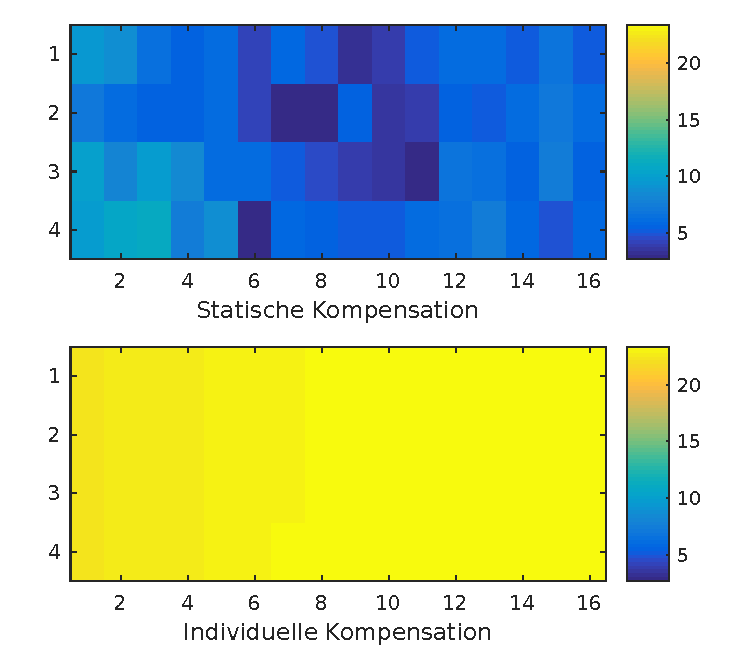
\includegraphics[width=\columnwidth]{fig/thermal_img_static_dyn.pdf}
	\caption{Vergleich der Sensorkompensation bei statischem und individuellem Ansatz}
	\label{fig:temp_ir:komp_vgl}
\end{figure}
Der Sensor kann Temperatur im Bereich von -20\,\textdegree{}C bis +300\,\textdegree{}C erfassen und darf bei einer Umgebungstemperatur zwischen -40\,\textdegree{}C und +85\,\textdegree{}C betrieben werden. Dieser große Temperaturbereich sollte jedes der Szenarien abdecken. Der Temperatursensor kommuniziert per \gls{I2C} Bus mit dem eingesetzten Raspberry Pi und stellt neben den Strahlungswerten auch Kompensationswerte in einem \gls{EEPROM} zur Verfügung.\\
Diese Kompensationswerte sind für eine genaue Messung entscheidend und werden vom Hersteller für jeden Sensor einzeln ermittelt. Zur Verdeutlichung der Zusammenhänge soll kurz die Methodik eines solchen Sensors umrissen werden. Jedes Pixel besteht aus einem Thermoelement mit einer sehr geringen thermischen Kapazität, welches von seiner Umgebung durch einen schlechten Wärmeleiter abgegrenzt ist, wie zum Beispiel Vakuum. Durch diese Maßnahmen nimmt das Pixel sehr schnell den Temperaturwert des zu beobachteten Gegenstandes an. Der Spannungswert eines solchen Thermoelements ist aber relativ zur Umgebungstemperatur zu sehen. Somit muss diese ($T_a$) ermittelt werden und in die tatsächliche Temperatur einfließen, es wird von Kaltstellenkompensation gesprochen. Der eigentliche Temperaturwert ergibt sich somit durch Addition der Umgebungstemperatur mit dem Wert des Thermoelements. Durch die thermische Isolation der Elemente reagieren diese sehr träge auf Änderungen der Umgebungstemperatur, somit eilt die Kaltstellenkompensation der eigentlichen relativen Temperatur des Elements voraus. Um das auszugleichen wird noch die Temperatur eines von der Außenwelt isolierten Elements ermittelt und fließt als Heißstellenkompensation ein. Diese beiden Werte werden für alle Elemente als gleich angenommen was aber nur näherungsweise richtig ist. Ein in der Mitte liegende Sensor nimmt die Umgebungstemperatur schneller an als einer am Rand. Das zum Beispiel wird durch einen Wert innerhalb des \gls{EEPROM} individuell pro Element kompensiert. Der Unterschied zwischen allgemeiner und individueller Kompensation wird in \autoref{fig:temp_ir:komp_vgl} dargestellt.
In der Abbildung ist zu sehen das die Werte der statischen Kompensation stärker Rauschen und mit einem allgemeinen Offset versehen sind, wie die der individuellen Kompensation. Die Notwendigkeit einer solchen ist für eine fehlerarme Erkennung notwendig.\\
Der Sensor benötigt für optimale Betriebszustände einer Versorgungsspannung von 2,6\,Volt. Da der Raspberry Pi nur 3.3\,Volt und 5.0\,Volt zur Verfügung stellt musste einer externe Platine erstellt werden. Diese beinhaltet auch den in \autoref{ssec:lichtsensor} beschriebenen Lichtsensor und ist in \autoref{fig:platine} dargestellt. 
\begin{figure}
	\centering
	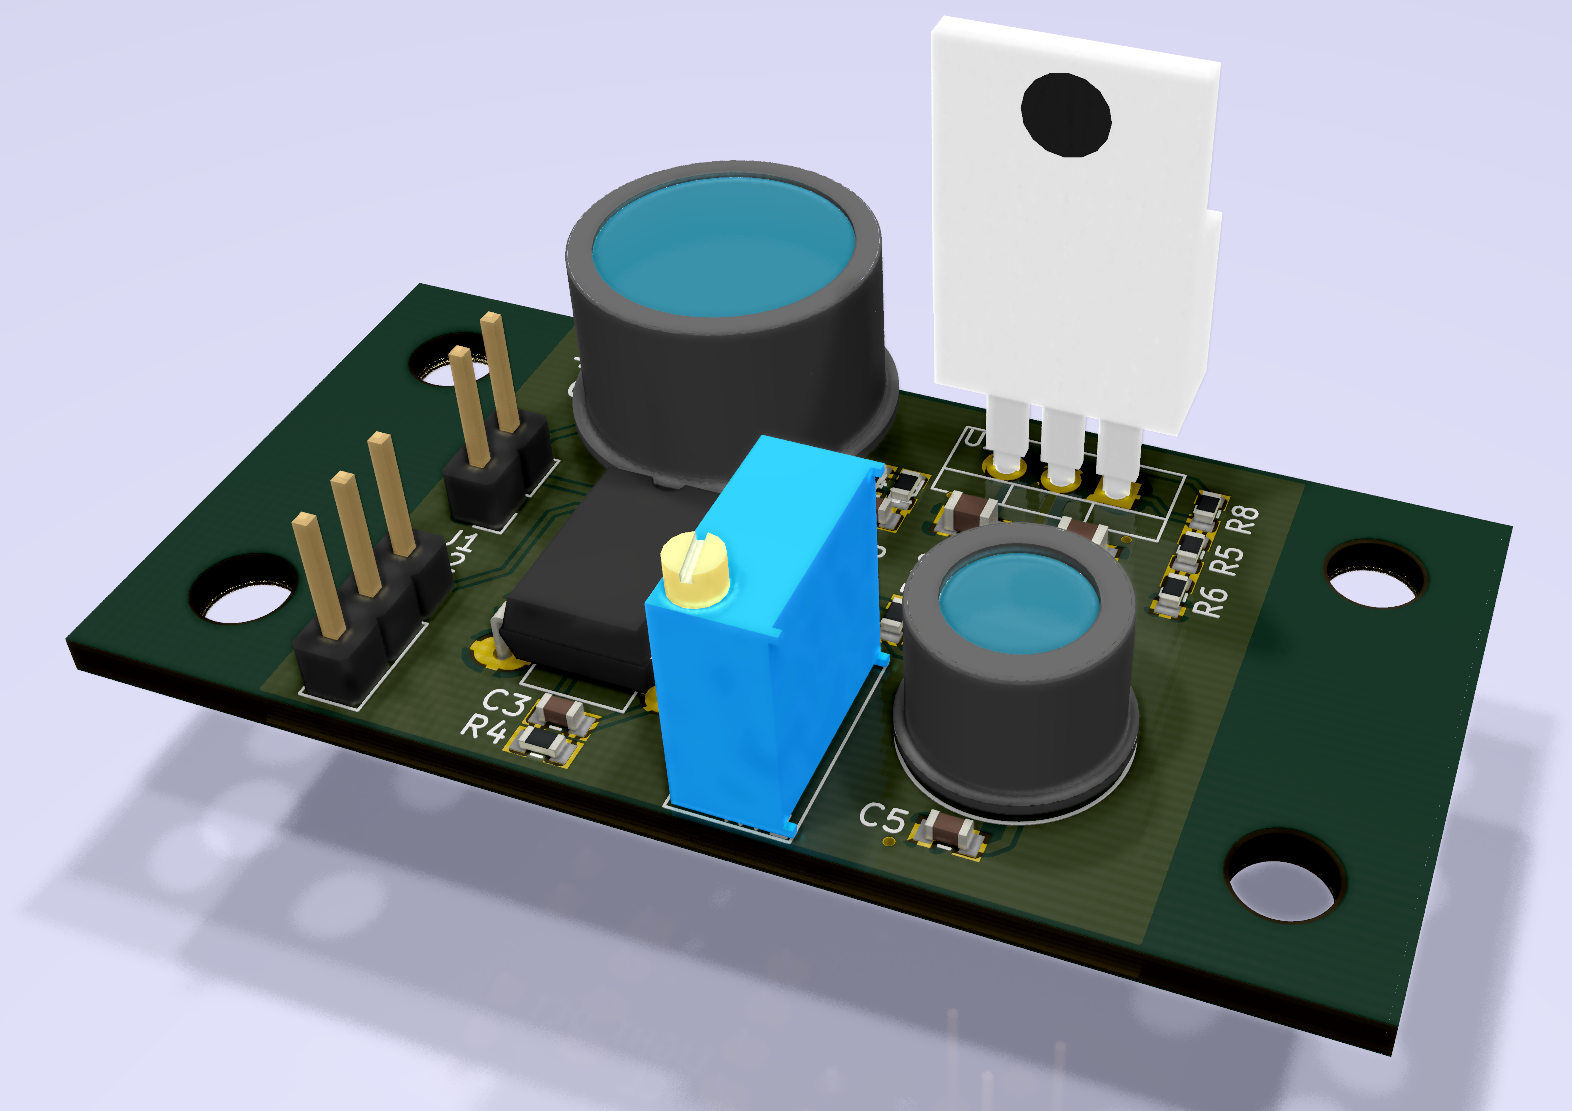
\includegraphics[width=\columnwidth]{fig/platine.png}
	\caption{Darstellung der Platine in 3D}
	\label{fig:platine}
\end{figure}
Die Platine stellt per \gls{LDO} eine Spannung von 2,6\,Volt bereit.\\
Die oben genannte Kompensation ist sehr zeitaufwendig. Durch mehrere Optimierungen mit numpy und Berechnung der Daten als Array war es möglich die Belastung des Raspberrys so weit zu reduzieren, das zirka 15 Frames pro Sekunden übertragen werden können. Der Sensor unterstützt bis zu 512 Frames pro Sekunde.
Nach der Kompensation stellt der Raspberry Pi die Daten per UDP in einem JSON Format zur Verfügung. Diese werden von einem OpenCV Skript angefordert. Dort wird auf das Rohbild ein Gaußscher Hintergrund / Vordergrund Segmentierungsalgorithmus zur Hintergrundentfernung angewendet. Von OpenCV wird dieser in der Klasse \emph{BackgroundSubtractorMOG2} zur Verfügung gestellt. Eine Schattenerkennung ist bei diesem deaktiviert, da nicht zum Sensor gerichtete thermische Abstrahlung nicht erkannt werden kann und die Notwendigkeit in diesem Fall nicht gegeben ist. Dieser Algorithmus funktioniert ohne weitere Anpassung sehr gut, hat aber das Problem des Einbrennens. Das heißt eine Wärmequelle, wie zum Beispiel eine Hand, geht nach einiger Zeit in den Hintergrund ein. Dies ist kein gewünschtes Verhalten, da unser System darauf ausgelegt ist, die Anwesenheit unabhängig von der Dauer zu erkennen. Dies wurde umgangen, indem Gegenstände die sich mehr als 3\,K von der Umgebungstemperatur unterscheiden, nur schwach gewichtet in den Lernprozess einfließen. Als Ergebnis wird somit ein 16x4 Pixel große Array erzeugt, dessen Elemente zwei Werte annehmen können - 0 für Hintergrund und 255 für den Vordergrund. Der Mittelwert dieses Arrays wird gegen einen Schwellwert verglichen und dann gegebenenfalls Alarm ausgelöst. Dieser ist vom Benutzer bestimmbar um möglichst flexibel auf gewünschte Wärmequellen reagieren zu können.

\subsection{Beschleunigungssensor}
Um detektieren zu können ob der Rucksack in Bewegung ist oder
still steht wird ein Beschleunigungssensor verwendet. Dieser
Sensor fertigt ein Akzelerogramm an. Das bedeutet, dass die
Geschwindigkeitszu- und abnahme kontinuierlich überwacht wird.
Dabei werden alle drei Raumachsen (X, Y u. Z) separat aufgezeichnet.
Wenn der Rucksack nun ruckartig vom Boden aufgehoben wird, erfährt er
eine Beschleunigung in Z-Richtung. Diese Abweichung vom
Normalzustand kann in der Auswertesoftware detektiert werden
und je nach Konfiguration zu einem Alarm führen. Dabei wird 
eine einfache Schwellwertfilterung auf den Sensor angewendet.
Um Bewegungen in alle Richtungen erkennen zu können werden natürlich
auch die aderen Raumachsen mit ausgeweretet.

\begin{figure}
\centering
  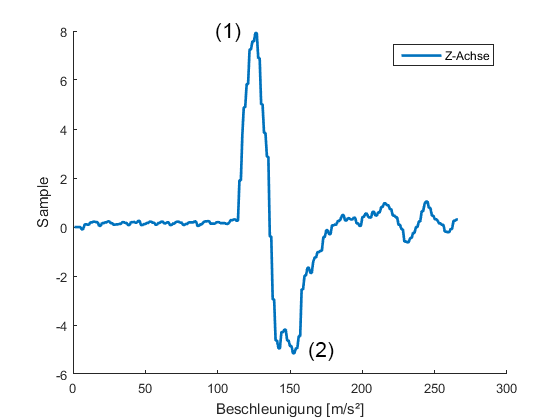
\includegraphics[width=0.9\columnwidth]{fig/accel_z.png}
  \caption{Akzelerogramm der Z-Achse beim Aufheben des Rucksacks}
  \label{fig:accel_z}
\end{figure}

Abbildung \ref{fig:accel_z} zeigt ein Akzelerogramm der Z-Achse,
das beim Aufheben des Rucksacks aufgezeichnet wurde. Der Peak (1)
in positiver Y-Richtung zeigt die Beschleunigung des Rucksackes
beim Aufheben an. Der Peak (2) in negativer Richtung zeigt das
Abremsen des Rucksacks an wenn die Aufhebebewegung abgeschlossen
ist. Der zu verwendende Schwellwert wurde in einer kleinen
Versuchsreihe expirementell bestimmt. Ein Schwellwert von \textit{1}
hat sich dabei als guter Wert herausgestellt. Dadurch kann
Sensorrauschen von einer tatsächlichen Bewegung unterschieden
werden. Der Erkennungsalgorithmus schlägt nur Alarm, wenn mehr
wie drei konsekutive Messungen über dem Schwellwert liegen. Damit
soll vermieden werden, dass Fehlmessungen einen Alarm auslösen.
Bei der Umsetzung des Prototypen wurde der BNO055 \cite{Bosch:BNO055}
von Bosch als Sensorsystem verwendet. Dieser wird im UART Modus
betrieben und über einen USB-TTL Adapter an das RaspberryPi
angebunden. Der Schritt über den USB Adapter ist nötig, da der
interne UART bereits für den GPS Empfänger verwendet wird.

\subsection{Lichtsensor}\label{ssec:lichtsensor}

\begin{itemize}
  \item Wozu? Welches Szenario?
  \item Einbindung des Sensors
\end{itemize}

\subsection{GPS}

\begin{itemize}
  \item Konzept: Save Zones
  \item Einbindung des Sensors
\end{itemize}

\section{Aktoren}

\subsection{Elektronisches Schloss}
Leider stand uns für unseren Prototypen kein elektronisches Schloss
zur Verfügung, weshalb der Schlosszustand mittels einer LED simuliert
wird. Nichts destotrotz gibt es bereits heute Vorhängeschlösser die
sich via Bluetooth ver- und entriegeln lassen \cite{MasterLock:Bluetooth}.
Es wäre durchaus denkbar so ein Schloss in die vorhandene Software
zu integrieren. Die Bluetooth Schnittstelle ließe sich über einen
Bluetooth USB Dongle am RaspberryPi nachrüsten. 

\subsection{Alarm}

\begin{itemize}
  \item warum akustischer Alarm?
  \item Wie umgesetzt?  
\end{itemize}

\section{Fazit und Ausblick}
Unser Prototyp zeigt, dass es durchaus möglich ist einen Rucksack zu
konstruieren, der einem Taschendieb das Leben schwer macht. Die Versuche
mit unvoreingenommenen Testpersonen haben durchweg positives Feedback
ergeben. Für ein Serienprodukt wäre der vorhandene Aufbau allerdings
nicht geeignet, da zuviel Transportvolumen von Elektronik und Sensorik
eingenommen werden würde. Durch weiteres Design eigener Platinen und einem 
Plattformwechsel sollte sich das aber leicht bewerkstelligen lassen.
Das hätte auch zur Folge, dass der Rucksack energiesparender arbeiten
würde und länger mit einer Akkufüllung auskommen würde, da das
RaspberryPi doch einen recht hohen Stromverbrauch aufzeigt \cite{Heise:RpiPower}.


\balance{}

% REFERENCES FORMAT
% References must be the same font size as other body text.
\bibliographystyle{SIGCHI-Reference-Format}
\bibliography{main}

\end{document}
